% Options for packages loaded elsewhere
\PassOptionsToPackage{unicode}{hyperref}
\PassOptionsToPackage{hyphens}{url}
%
\documentclass[
]{article}
\usepackage{amsmath,amssymb}
\usepackage{iftex}
\ifPDFTeX
  \usepackage[T1]{fontenc}
  \usepackage[utf8]{inputenc}
  \usepackage{textcomp} % provide euro and other symbols
\else % if luatex or xetex
  \usepackage{unicode-math} % this also loads fontspec
  \defaultfontfeatures{Scale=MatchLowercase}
  \defaultfontfeatures[\rmfamily]{Ligatures=TeX,Scale=1}
\fi
\usepackage{lmodern}
\ifPDFTeX\else
  % xetex/luatex font selection
\fi
% Use upquote if available, for straight quotes in verbatim environments
\IfFileExists{upquote.sty}{\usepackage{upquote}}{}
\IfFileExists{microtype.sty}{% use microtype if available
  \usepackage[]{microtype}
  \UseMicrotypeSet[protrusion]{basicmath} % disable protrusion for tt fonts
}{}
\makeatletter
\@ifundefined{KOMAClassName}{% if non-KOMA class
  \IfFileExists{parskip.sty}{%
    \usepackage{parskip}
  }{% else
    \setlength{\parindent}{0pt}
    \setlength{\parskip}{6pt plus 2pt minus 1pt}}
}{% if KOMA class
  \KOMAoptions{parskip=half}}
\makeatother
\usepackage{xcolor}
\usepackage[margin=1in]{geometry}
\usepackage{color}
\usepackage{fancyvrb}
\newcommand{\VerbBar}{|}
\newcommand{\VERB}{\Verb[commandchars=\\\{\}]}
\DefineVerbatimEnvironment{Highlighting}{Verbatim}{commandchars=\\\{\}}
% Add ',fontsize=\small' for more characters per line
\usepackage{framed}
\definecolor{shadecolor}{RGB}{248,248,248}
\newenvironment{Shaded}{\begin{snugshade}}{\end{snugshade}}
\newcommand{\AlertTok}[1]{\textcolor[rgb]{0.94,0.16,0.16}{#1}}
\newcommand{\AnnotationTok}[1]{\textcolor[rgb]{0.56,0.35,0.01}{\textbf{\textit{#1}}}}
\newcommand{\AttributeTok}[1]{\textcolor[rgb]{0.13,0.29,0.53}{#1}}
\newcommand{\BaseNTok}[1]{\textcolor[rgb]{0.00,0.00,0.81}{#1}}
\newcommand{\BuiltInTok}[1]{#1}
\newcommand{\CharTok}[1]{\textcolor[rgb]{0.31,0.60,0.02}{#1}}
\newcommand{\CommentTok}[1]{\textcolor[rgb]{0.56,0.35,0.01}{\textit{#1}}}
\newcommand{\CommentVarTok}[1]{\textcolor[rgb]{0.56,0.35,0.01}{\textbf{\textit{#1}}}}
\newcommand{\ConstantTok}[1]{\textcolor[rgb]{0.56,0.35,0.01}{#1}}
\newcommand{\ControlFlowTok}[1]{\textcolor[rgb]{0.13,0.29,0.53}{\textbf{#1}}}
\newcommand{\DataTypeTok}[1]{\textcolor[rgb]{0.13,0.29,0.53}{#1}}
\newcommand{\DecValTok}[1]{\textcolor[rgb]{0.00,0.00,0.81}{#1}}
\newcommand{\DocumentationTok}[1]{\textcolor[rgb]{0.56,0.35,0.01}{\textbf{\textit{#1}}}}
\newcommand{\ErrorTok}[1]{\textcolor[rgb]{0.64,0.00,0.00}{\textbf{#1}}}
\newcommand{\ExtensionTok}[1]{#1}
\newcommand{\FloatTok}[1]{\textcolor[rgb]{0.00,0.00,0.81}{#1}}
\newcommand{\FunctionTok}[1]{\textcolor[rgb]{0.13,0.29,0.53}{\textbf{#1}}}
\newcommand{\ImportTok}[1]{#1}
\newcommand{\InformationTok}[1]{\textcolor[rgb]{0.56,0.35,0.01}{\textbf{\textit{#1}}}}
\newcommand{\KeywordTok}[1]{\textcolor[rgb]{0.13,0.29,0.53}{\textbf{#1}}}
\newcommand{\NormalTok}[1]{#1}
\newcommand{\OperatorTok}[1]{\textcolor[rgb]{0.81,0.36,0.00}{\textbf{#1}}}
\newcommand{\OtherTok}[1]{\textcolor[rgb]{0.56,0.35,0.01}{#1}}
\newcommand{\PreprocessorTok}[1]{\textcolor[rgb]{0.56,0.35,0.01}{\textit{#1}}}
\newcommand{\RegionMarkerTok}[1]{#1}
\newcommand{\SpecialCharTok}[1]{\textcolor[rgb]{0.81,0.36,0.00}{\textbf{#1}}}
\newcommand{\SpecialStringTok}[1]{\textcolor[rgb]{0.31,0.60,0.02}{#1}}
\newcommand{\StringTok}[1]{\textcolor[rgb]{0.31,0.60,0.02}{#1}}
\newcommand{\VariableTok}[1]{\textcolor[rgb]{0.00,0.00,0.00}{#1}}
\newcommand{\VerbatimStringTok}[1]{\textcolor[rgb]{0.31,0.60,0.02}{#1}}
\newcommand{\WarningTok}[1]{\textcolor[rgb]{0.56,0.35,0.01}{\textbf{\textit{#1}}}}
\usepackage{graphicx}
\makeatletter
\def\maxwidth{\ifdim\Gin@nat@width>\linewidth\linewidth\else\Gin@nat@width\fi}
\def\maxheight{\ifdim\Gin@nat@height>\textheight\textheight\else\Gin@nat@height\fi}
\makeatother
% Scale images if necessary, so that they will not overflow the page
% margins by default, and it is still possible to overwrite the defaults
% using explicit options in \includegraphics[width, height, ...]{}
\setkeys{Gin}{width=\maxwidth,height=\maxheight,keepaspectratio}
% Set default figure placement to htbp
\makeatletter
\def\fps@figure{htbp}
\makeatother
\setlength{\emergencystretch}{3em} % prevent overfull lines
\providecommand{\tightlist}{%
  \setlength{\itemsep}{0pt}\setlength{\parskip}{0pt}}
\setcounter{secnumdepth}{-\maxdimen} % remove section numbering
\ifLuaTeX
  \usepackage{selnolig}  % disable illegal ligatures
\fi
\usepackage{bookmark}
\IfFileExists{xurl.sty}{\usepackage{xurl}}{} % add URL line breaks if available
\urlstyle{same}
\hypersetup{
  hidelinks,
  pdfcreator={LaTeX via pandoc}}

\author{}
\date{\vspace{-2.5em}}

\begin{document}

\subsection{1. Graphical models}\label{graphical-models}

\begin{enumerate}
\def\labelenumi{\arabic{enumi})}
\tightlist
\item
\end{enumerate}

\begin{Shaded}
\begin{Highlighting}[]
\FunctionTok{library}\NormalTok{(bnlearn)}
\FunctionTok{library}\NormalTok{(gRain)}
\end{Highlighting}
\end{Shaded}

\begin{verbatim}
## Loading required package: gRbase
\end{verbatim}

\begin{verbatim}
## 
## Attaching package: 'gRbase'
\end{verbatim}

\begin{verbatim}
## The following objects are masked from 'package:bnlearn':
## 
##     ancestors, children, nodes, parents
\end{verbatim}

\begin{Shaded}
\begin{Highlighting}[]
\NormalTok{dag }\OtherTok{=} \FunctionTok{model2network}\NormalTok{(}\StringTok{"[C][D|C][A|C][Y|A:C]"}\NormalTok{)}

\FunctionTok{graphviz.plot}\NormalTok{(dag)}
\end{Highlighting}
\end{Shaded}

\begin{verbatim}
## Loading required namespace: Rgraphviz
\end{verbatim}

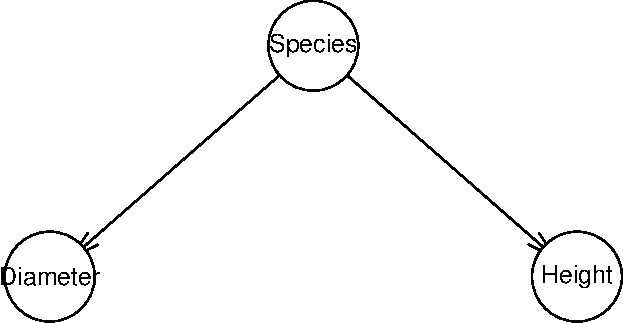
\includegraphics{oct2020_files/figure-latex/unnamed-chunk-1-1.pdf}

\begin{enumerate}
\def\labelenumi{\arabic{enumi})}
\setcounter{enumi}{1}
\tightlist
\item
\end{enumerate}

\begin{Shaded}
\begin{Highlighting}[]
\NormalTok{countC\_ND }\OtherTok{=} \DecValTok{0}
\NormalTok{countD\_NC }\OtherTok{=} \DecValTok{0}
\ControlFlowTok{for}\NormalTok{ (i }\ControlFlowTok{in} \DecValTok{1}\SpecialCharTok{:}\DecValTok{1000}\NormalTok{) \{}
\NormalTok{  dag }\OtherTok{=} \FunctionTok{model2network}\NormalTok{(}\StringTok{"[C][D|C][A|C][Y|A:C]"}\NormalTok{)}
  \CommentTok{\# C}
\NormalTok{  s }\OtherTok{=} \FunctionTok{runif}\NormalTok{(}\DecValTok{1}\NormalTok{)}
\NormalTok{  cptC }\OtherTok{=} \FunctionTok{c}\NormalTok{(s, }\DecValTok{1}\SpecialCharTok{{-}}\NormalTok{s)}
  \FunctionTok{dim}\NormalTok{(cptC) }\OtherTok{=} \FunctionTok{c}\NormalTok{(}\DecValTok{2}\NormalTok{)}
  \FunctionTok{dimnames}\NormalTok{(cptC) }\OtherTok{=} \FunctionTok{list}\NormalTok{(}\AttributeTok{C =} \FunctionTok{c}\NormalTok{(}\StringTok{"C1"}\NormalTok{, }\StringTok{"C0"}\NormalTok{))}

  \CommentTok{\# D | C}
\NormalTok{  s1 }\OtherTok{=} \FunctionTok{runif}\NormalTok{(}\DecValTok{1}\NormalTok{)}
\NormalTok{  s2 }\OtherTok{=} \FunctionTok{runif}\NormalTok{(}\DecValTok{1}\NormalTok{)}
\NormalTok{  cptD }\OtherTok{=} \FunctionTok{matrix}\NormalTok{(}\FunctionTok{c}\NormalTok{(s1, }\DecValTok{1}\SpecialCharTok{{-}}\NormalTok{s1,  }
\NormalTok{                 s2, }\DecValTok{1}\SpecialCharTok{{-}}\NormalTok{s2),}
               \AttributeTok{nrow =} \DecValTok{2}\NormalTok{)}
  \FunctionTok{dimnames}\NormalTok{(cptD) }\OtherTok{=} \FunctionTok{list}\NormalTok{(}\AttributeTok{D =} \FunctionTok{c}\NormalTok{(}\StringTok{"D1"}\NormalTok{, }\StringTok{"D0"}\NormalTok{), }\AttributeTok{C =} \FunctionTok{c}\NormalTok{(}\StringTok{"C1"}\NormalTok{, }\StringTok{"C0"}\NormalTok{))}

   \CommentTok{\# A | C}
\NormalTok{  s1 }\OtherTok{=} \FunctionTok{runif}\NormalTok{(}\DecValTok{1}\NormalTok{)}
\NormalTok{  s2 }\OtherTok{=} \FunctionTok{runif}\NormalTok{(}\DecValTok{1}\NormalTok{)}
\NormalTok{  cptA }\OtherTok{=} \FunctionTok{matrix}\NormalTok{(}\FunctionTok{c}\NormalTok{(s1, }\DecValTok{1}\SpecialCharTok{{-}}\NormalTok{s1,  }
\NormalTok{                 s2, }\DecValTok{1}\SpecialCharTok{{-}}\NormalTok{s2),}
               \AttributeTok{nrow =} \DecValTok{2}\NormalTok{)}
  \FunctionTok{dimnames}\NormalTok{(cptA) }\OtherTok{=} \FunctionTok{list}\NormalTok{(}\AttributeTok{A =} \FunctionTok{c}\NormalTok{(}\StringTok{"A1"}\NormalTok{, }\StringTok{"A0"}\NormalTok{), }\AttributeTok{C =} \FunctionTok{c}\NormalTok{(}\StringTok{"C1"}\NormalTok{, }\StringTok{"C0"}\NormalTok{))}
  
     \CommentTok{\# Y | A,C}
\NormalTok{  s1 }\OtherTok{=} \FunctionTok{runif}\NormalTok{(}\DecValTok{1}\NormalTok{)}
\NormalTok{  s2 }\OtherTok{=} \FunctionTok{runif}\NormalTok{(}\DecValTok{1}\NormalTok{)}
\NormalTok{  s3 }\OtherTok{=} \FunctionTok{runif}\NormalTok{(}\DecValTok{1}\NormalTok{)}
\NormalTok{  s4 }\OtherTok{=} \FunctionTok{runif}\NormalTok{(}\DecValTok{1}\NormalTok{)}
\NormalTok{  cptY }\OtherTok{=} \FunctionTok{matrix}\NormalTok{(}\FunctionTok{c}\NormalTok{(s1,}\DecValTok{1}\SpecialCharTok{{-}}\NormalTok{s1,}
\NormalTok{                  s2,}\DecValTok{1}\SpecialCharTok{{-}}\NormalTok{s2,}
\NormalTok{                  s3,}\DecValTok{1}\SpecialCharTok{{-}}\NormalTok{s3,}
\NormalTok{                  s4,}\DecValTok{1}\SpecialCharTok{{-}}\NormalTok{s4),}
\NormalTok{                )}
  \FunctionTok{dim}\NormalTok{(cptY) }\OtherTok{=} \FunctionTok{c}\NormalTok{(}\DecValTok{2}\NormalTok{,}\DecValTok{2}\NormalTok{,}\DecValTok{2}\NormalTok{)}
  \FunctionTok{dimnames}\NormalTok{(cptY) }\OtherTok{=} \FunctionTok{list}\NormalTok{(}\AttributeTok{Y =} \FunctionTok{c}\NormalTok{(}\StringTok{"Y1"}\NormalTok{, }\StringTok{"Y0"}\NormalTok{), }\AttributeTok{A =} \FunctionTok{c}\NormalTok{(}\StringTok{"A1"}\NormalTok{, }\StringTok{"A0"}\NormalTok{), }\AttributeTok{C =} \FunctionTok{c}\NormalTok{(}\StringTok{"C1"}\NormalTok{, }\StringTok{"C0"}\NormalTok{))}

\NormalTok{  fit }\OtherTok{=} \FunctionTok{custom.fit}\NormalTok{(dag, }\FunctionTok{list}\NormalTok{(}\AttributeTok{C =}\NormalTok{ cptC,}\AttributeTok{D =}\NormalTok{ cptD,}\AttributeTok{A =}\NormalTok{ cptA, }\AttributeTok{Y =}\NormalTok{ cptY))}
\NormalTok{  model }\OtherTok{=} \FunctionTok{compile}\NormalTok{(}\FunctionTok{as.grain}\NormalTok{(fit))}
  
  \CommentTok{\# for p(y|a,c)}
\NormalTok{  Y1\_A1C1 }\OtherTok{\textless{}{-}} \FunctionTok{querygrain}\NormalTok{(}\FunctionTok{setEvidence}\NormalTok{(}\AttributeTok{object =}\NormalTok{ model, }\AttributeTok{nodes =} \FunctionTok{c}\NormalTok{(}\StringTok{"A"}\NormalTok{, }\StringTok{"C"}\NormalTok{), }\AttributeTok{states =} \FunctionTok{c}\NormalTok{(}\StringTok{"A1"}\NormalTok{, }\StringTok{"C1"}\NormalTok{)),}\AttributeTok{nodes =} \StringTok{"Y"}\NormalTok{)}\SpecialCharTok{$}\NormalTok{Y[}\DecValTok{1}\NormalTok{]}
\NormalTok{  Y1\_A1C0 }\OtherTok{\textless{}{-}} \FunctionTok{querygrain}\NormalTok{(}\FunctionTok{setEvidence}\NormalTok{(}\AttributeTok{object =}\NormalTok{ model, }\AttributeTok{nodes =} \FunctionTok{c}\NormalTok{(}\StringTok{"A"}\NormalTok{, }\StringTok{"C"}\NormalTok{), }\AttributeTok{states =} \FunctionTok{c}\NormalTok{(}\StringTok{"A1"}\NormalTok{, }\StringTok{"C0"}\NormalTok{)),}\AttributeTok{nodes =} \StringTok{"Y"}\NormalTok{)}\SpecialCharTok{$}\NormalTok{Y[}\DecValTok{1}\NormalTok{]}
\NormalTok{  Y1\_A0C1 }\OtherTok{\textless{}{-}} \FunctionTok{querygrain}\NormalTok{(}\FunctionTok{setEvidence}\NormalTok{(}\AttributeTok{object =}\NormalTok{ model, }\AttributeTok{nodes =} \FunctionTok{c}\NormalTok{(}\StringTok{"A"}\NormalTok{, }\StringTok{"C"}\NormalTok{), }\AttributeTok{states =} \FunctionTok{c}\NormalTok{(}\StringTok{"A0"}\NormalTok{, }\StringTok{"C1"}\NormalTok{)),}\AttributeTok{nodes =} \StringTok{"Y"}\NormalTok{)}\SpecialCharTok{$}\NormalTok{Y[}\DecValTok{1}\NormalTok{]}
\NormalTok{  Y1\_A0C0 }\OtherTok{\textless{}{-}} \FunctionTok{querygrain}\NormalTok{(}\FunctionTok{setEvidence}\NormalTok{(}\AttributeTok{object =}\NormalTok{ model, }\AttributeTok{nodes =} \FunctionTok{c}\NormalTok{(}\StringTok{"A"}\NormalTok{, }\StringTok{"C"}\NormalTok{), }\AttributeTok{states =} \FunctionTok{c}\NormalTok{(}\StringTok{"A0"}\NormalTok{, }\StringTok{"C0"}\NormalTok{)),}\AttributeTok{nodes =} \StringTok{"Y"}\NormalTok{)}\SpecialCharTok{$}\NormalTok{Y[}\DecValTok{1}\NormalTok{]}
  
  \CommentTok{\# for p(y|a,d)}
\NormalTok{  Y1\_A1D1 }\OtherTok{\textless{}{-}} \FunctionTok{querygrain}\NormalTok{(}\FunctionTok{setEvidence}\NormalTok{(}\AttributeTok{object =}\NormalTok{ model, }\AttributeTok{nodes =} \FunctionTok{c}\NormalTok{(}\StringTok{"A"}\NormalTok{, }\StringTok{"D"}\NormalTok{), }\AttributeTok{states =} \FunctionTok{c}\NormalTok{(}\StringTok{"A1"}\NormalTok{, }\StringTok{"D1"}\NormalTok{)),}\AttributeTok{nodes =} \StringTok{"Y"}\NormalTok{)}\SpecialCharTok{$}\NormalTok{Y[}\DecValTok{1}\NormalTok{]}
\NormalTok{  Y1\_A1D0 }\OtherTok{\textless{}{-}} \FunctionTok{querygrain}\NormalTok{(}\FunctionTok{setEvidence}\NormalTok{(}\AttributeTok{object =}\NormalTok{ model, }\AttributeTok{nodes =} \FunctionTok{c}\NormalTok{(}\StringTok{"A"}\NormalTok{, }\StringTok{"D"}\NormalTok{), }\AttributeTok{states =} \FunctionTok{c}\NormalTok{(}\StringTok{"A1"}\NormalTok{, }\StringTok{"D0"}\NormalTok{)),}\AttributeTok{nodes =} \StringTok{"Y"}\NormalTok{)}\SpecialCharTok{$}\NormalTok{Y[}\DecValTok{1}\NormalTok{]}
\NormalTok{  Y1\_A0D1 }\OtherTok{\textless{}{-}} \FunctionTok{querygrain}\NormalTok{(}\FunctionTok{setEvidence}\NormalTok{(}\AttributeTok{object =}\NormalTok{ model, }\AttributeTok{nodes =} \FunctionTok{c}\NormalTok{(}\StringTok{"A"}\NormalTok{, }\StringTok{"D"}\NormalTok{), }\AttributeTok{states =} \FunctionTok{c}\NormalTok{(}\StringTok{"A0"}\NormalTok{, }\StringTok{"D1"}\NormalTok{)),}\AttributeTok{nodes =} \StringTok{"Y"}\NormalTok{)}\SpecialCharTok{$}\NormalTok{Y[}\DecValTok{1}\NormalTok{]}
\NormalTok{  Y1\_A0D0 }\OtherTok{\textless{}{-}} \FunctionTok{querygrain}\NormalTok{(}\FunctionTok{setEvidence}\NormalTok{(}\AttributeTok{object =}\NormalTok{ model, }\AttributeTok{nodes =} \FunctionTok{c}\NormalTok{(}\StringTok{"A"}\NormalTok{, }\StringTok{"D"}\NormalTok{), }\AttributeTok{states =} \FunctionTok{c}\NormalTok{(}\StringTok{"A0"}\NormalTok{, }\StringTok{"D0"}\NormalTok{)),}\AttributeTok{nodes =} \StringTok{"Y"}\NormalTok{)}\SpecialCharTok{$}\NormalTok{Y[}\DecValTok{1}\NormalTok{]}
 
  \ControlFlowTok{if}\NormalTok{(Y1\_A1C1 }\SpecialCharTok{\textgreater{}=}\NormalTok{ Y1\_A1C0 }\SpecialCharTok{\&\&}\NormalTok{ Y1\_A0C1 }\SpecialCharTok{\textgreater{}=}\NormalTok{ Y1\_A0C0)\{}
    \ControlFlowTok{if}\NormalTok{(Y1\_A1C1 }\SpecialCharTok{\textless{}=}\NormalTok{ Y1\_A1C0 }\SpecialCharTok{\&\&}\NormalTok{ Y1\_A0C1 }\SpecialCharTok{\textless{}=}\NormalTok{ Y1\_A0C0)\{}
\NormalTok{      monotoneC }\OtherTok{=} \ConstantTok{TRUE}
\NormalTok{    \}}
\NormalTok{    \} }\ControlFlowTok{else}\NormalTok{ \{}
\NormalTok{    monotoneC }\OtherTok{=} \ConstantTok{FALSE}
\NormalTok{  \}}
 
\NormalTok{      monotoneD }\OtherTok{=} \ConstantTok{FALSE}
   \ControlFlowTok{if}\NormalTok{(Y1\_A1D1 }\SpecialCharTok{\textgreater{}=}\NormalTok{ Y1\_A1D0 }\SpecialCharTok{\&\&}\NormalTok{ Y1\_A0D1 }\SpecialCharTok{\textgreater{}=}\NormalTok{ Y1\_A0D0)\{}
    \ControlFlowTok{if}\NormalTok{(Y1\_A1D1 }\SpecialCharTok{\textless{}=}\NormalTok{ Y1\_A1D0 }\SpecialCharTok{\&\&}\NormalTok{ Y1\_A0D1 }\SpecialCharTok{\textless{}=}\NormalTok{ Y1\_A0D0)\{}
\NormalTok{      monotoneD }\OtherTok{=} \ConstantTok{TRUE}
\NormalTok{    \}}
\NormalTok{    \} }\ControlFlowTok{else}\NormalTok{ \{}
\NormalTok{    monotoneD }\OtherTok{=} \ConstantTok{FALSE}
\NormalTok{  \}}
 
 
  \ControlFlowTok{if}\NormalTok{(monotoneC }\SpecialCharTok{\&\&} \SpecialCharTok{!}\NormalTok{monotoneD)\{}
\NormalTok{    countC\_ND }\OtherTok{=}\NormalTok{ countC\_ND }\SpecialCharTok{+}\DecValTok{1}
\NormalTok{  \}}\ControlFlowTok{else} \ControlFlowTok{if}\NormalTok{(}\SpecialCharTok{!}\NormalTok{monotoneC }\SpecialCharTok{\&\&}\NormalTok{ monotoneD)\{}
\NormalTok{    countD\_NC }\OtherTok{=}\NormalTok{ countD\_NC }\SpecialCharTok{+}\DecValTok{1} 
\NormalTok{  \}}
\NormalTok{\}}

\NormalTok{countC\_ND}
\end{Highlighting}
\end{Shaded}

\begin{verbatim}
## [1] 0
\end{verbatim}

\begin{Shaded}
\begin{Highlighting}[]
\NormalTok{countD\_NC}
\end{Highlighting}
\end{Shaded}

\begin{verbatim}
## [1] 0
\end{verbatim}

\begin{enumerate}
\def\labelenumi{\roman{enumi})}
\item
  how many of parametrisation result in p(\textbar a,c) is monotone in C
  but p(y\textbar a,d) is not monotone in d
\item
  p(y∣a, d) is monotone in D but p(y∣a, c) is not monotone in C
\end{enumerate}

\begin{Shaded}
\begin{Highlighting}[]
\FunctionTok{set.seed}\NormalTok{(}\DecValTok{1234}\NormalTok{)}
\FunctionTok{library}\NormalTok{(ggplot2)}

\NormalTok{arrows }\OtherTok{\textless{}{-}} \FunctionTok{c}\NormalTok{(}\StringTok{"\^{}"}\NormalTok{, }\StringTok{"\textgreater{}"}\NormalTok{, }\StringTok{"v"}\NormalTok{, }\StringTok{"\textless{}"}\NormalTok{)}
\NormalTok{action\_deltas }\OtherTok{\textless{}{-}} \FunctionTok{list}\NormalTok{(}\FunctionTok{c}\NormalTok{(}\DecValTok{1}\NormalTok{,}\DecValTok{0}\NormalTok{), }\CommentTok{\# up}
                      \FunctionTok{c}\NormalTok{(}\DecValTok{0}\NormalTok{,}\DecValTok{1}\NormalTok{), }\CommentTok{\# right}
                      \FunctionTok{c}\NormalTok{(}\SpecialCharTok{{-}}\DecValTok{1}\NormalTok{,}\DecValTok{0}\NormalTok{), }\CommentTok{\# down}
                      \FunctionTok{c}\NormalTok{(}\DecValTok{0}\NormalTok{,}\SpecialCharTok{{-}}\DecValTok{1}\NormalTok{)) }\CommentTok{\# left}

\NormalTok{vis\_environment }\OtherTok{\textless{}{-}} \ControlFlowTok{function}\NormalTok{(}\AttributeTok{iterations=}\DecValTok{0}\NormalTok{, }\AttributeTok{epsilon =} \FloatTok{0.5}\NormalTok{, }\AttributeTok{alpha =} \FloatTok{0.1}\NormalTok{, }\AttributeTok{gamma =} \FloatTok{0.95}\NormalTok{, }\AttributeTok{beta =} \DecValTok{0}\NormalTok{)\{}

\NormalTok{  df }\OtherTok{\textless{}{-}} \FunctionTok{expand.grid}\NormalTok{(}\AttributeTok{x=}\DecValTok{1}\SpecialCharTok{:}\NormalTok{H,}\AttributeTok{y=}\DecValTok{1}\SpecialCharTok{:}\NormalTok{W)}
\NormalTok{  foo }\OtherTok{\textless{}{-}} \FunctionTok{mapply}\NormalTok{(}\ControlFlowTok{function}\NormalTok{(x,y) }\FunctionTok{ifelse}\NormalTok{(reward\_map[x,y] }\SpecialCharTok{==} \DecValTok{0}\NormalTok{,q\_table[x,y,}\DecValTok{1}\NormalTok{],}\ConstantTok{NA}\NormalTok{),df}\SpecialCharTok{$}\NormalTok{x,df}\SpecialCharTok{$}\NormalTok{y)}
\NormalTok{  df}\SpecialCharTok{$}\NormalTok{val1 }\OtherTok{\textless{}{-}} \FunctionTok{as.vector}\NormalTok{(}\FunctionTok{round}\NormalTok{(foo, }\DecValTok{2}\NormalTok{))}
\NormalTok{  foo }\OtherTok{\textless{}{-}} \FunctionTok{mapply}\NormalTok{(}\ControlFlowTok{function}\NormalTok{(x,y) }\FunctionTok{ifelse}\NormalTok{(reward\_map[x,y] }\SpecialCharTok{==} \DecValTok{0}\NormalTok{,q\_table[x,y,}\DecValTok{2}\NormalTok{],}\ConstantTok{NA}\NormalTok{),df}\SpecialCharTok{$}\NormalTok{x,df}\SpecialCharTok{$}\NormalTok{y)}
\NormalTok{  df}\SpecialCharTok{$}\NormalTok{val2 }\OtherTok{\textless{}{-}} \FunctionTok{as.vector}\NormalTok{(}\FunctionTok{round}\NormalTok{(foo, }\DecValTok{2}\NormalTok{))}
\NormalTok{  foo }\OtherTok{\textless{}{-}} \FunctionTok{mapply}\NormalTok{(}\ControlFlowTok{function}\NormalTok{(x,y) }\FunctionTok{ifelse}\NormalTok{(reward\_map[x,y] }\SpecialCharTok{==} \DecValTok{0}\NormalTok{,q\_table[x,y,}\DecValTok{3}\NormalTok{],}\ConstantTok{NA}\NormalTok{),df}\SpecialCharTok{$}\NormalTok{x,df}\SpecialCharTok{$}\NormalTok{y)}
\NormalTok{  df}\SpecialCharTok{$}\NormalTok{val3 }\OtherTok{\textless{}{-}} \FunctionTok{as.vector}\NormalTok{(}\FunctionTok{round}\NormalTok{(foo, }\DecValTok{2}\NormalTok{))}
\NormalTok{  foo }\OtherTok{\textless{}{-}} \FunctionTok{mapply}\NormalTok{(}\ControlFlowTok{function}\NormalTok{(x,y) }\FunctionTok{ifelse}\NormalTok{(reward\_map[x,y] }\SpecialCharTok{==} \DecValTok{0}\NormalTok{,q\_table[x,y,}\DecValTok{4}\NormalTok{],}\ConstantTok{NA}\NormalTok{),df}\SpecialCharTok{$}\NormalTok{x,df}\SpecialCharTok{$}\NormalTok{y)}
\NormalTok{  df}\SpecialCharTok{$}\NormalTok{val4 }\OtherTok{\textless{}{-}} \FunctionTok{as.vector}\NormalTok{(}\FunctionTok{round}\NormalTok{(foo, }\DecValTok{2}\NormalTok{))}
\NormalTok{  foo }\OtherTok{\textless{}{-}} \FunctionTok{mapply}\NormalTok{(}\ControlFlowTok{function}\NormalTok{(x,y) }
    \FunctionTok{ifelse}\NormalTok{(reward\_map[x,y] }\SpecialCharTok{==} \DecValTok{0}\NormalTok{,arrows[}\FunctionTok{GreedyPolicy}\NormalTok{(x,y)],reward\_map[x,y]),df}\SpecialCharTok{$}\NormalTok{x,df}\SpecialCharTok{$}\NormalTok{y)}
\NormalTok{  df}\SpecialCharTok{$}\NormalTok{val5 }\OtherTok{\textless{}{-}} \FunctionTok{as.vector}\NormalTok{(foo)}
\NormalTok{  foo }\OtherTok{\textless{}{-}} \FunctionTok{mapply}\NormalTok{(}\ControlFlowTok{function}\NormalTok{(x,y) }\FunctionTok{ifelse}\NormalTok{(reward\_map[x,y] }\SpecialCharTok{==} \DecValTok{0}\NormalTok{,}\FunctionTok{max}\NormalTok{(q\_table[x,y,]),}
                                     \FunctionTok{ifelse}\NormalTok{(reward\_map[x,y]}\SpecialCharTok{\textless{}}\DecValTok{0}\NormalTok{,}\ConstantTok{NA}\NormalTok{,reward\_map[x,y])),df}\SpecialCharTok{$}\NormalTok{x,df}\SpecialCharTok{$}\NormalTok{y)}
\NormalTok{  df}\SpecialCharTok{$}\NormalTok{val6 }\OtherTok{\textless{}{-}} \FunctionTok{as.vector}\NormalTok{(foo)}
  
  \FunctionTok{print}\NormalTok{(}\FunctionTok{ggplot}\NormalTok{(df,}\FunctionTok{aes}\NormalTok{(}\AttributeTok{x =}\NormalTok{ y,}\AttributeTok{y =}\NormalTok{ x)) }\SpecialCharTok{+}
          \FunctionTok{scale\_fill\_gradient}\NormalTok{(}\AttributeTok{low =} \StringTok{"white"}\NormalTok{, }\AttributeTok{high =} \StringTok{"green"}\NormalTok{, }\AttributeTok{na.value =} \StringTok{"red"}\NormalTok{, }\AttributeTok{name =} \StringTok{""}\NormalTok{) }\SpecialCharTok{+}
          \FunctionTok{geom\_tile}\NormalTok{(}\FunctionTok{aes}\NormalTok{(}\AttributeTok{fill=}\NormalTok{val6)) }\SpecialCharTok{+}
          \FunctionTok{geom\_text}\NormalTok{(}\FunctionTok{aes}\NormalTok{(}\AttributeTok{label =}\NormalTok{ val1),}\AttributeTok{size =} \DecValTok{4}\NormalTok{,}\AttributeTok{nudge\_y =}\NormalTok{ .}\DecValTok{35}\NormalTok{,}\AttributeTok{na.rm =} \ConstantTok{TRUE}\NormalTok{) }\SpecialCharTok{+}
          \FunctionTok{geom\_text}\NormalTok{(}\FunctionTok{aes}\NormalTok{(}\AttributeTok{label =}\NormalTok{ val2),}\AttributeTok{size =} \DecValTok{4}\NormalTok{,}\AttributeTok{nudge\_x =}\NormalTok{ .}\DecValTok{35}\NormalTok{,}\AttributeTok{na.rm =} \ConstantTok{TRUE}\NormalTok{) }\SpecialCharTok{+}
          \FunctionTok{geom\_text}\NormalTok{(}\FunctionTok{aes}\NormalTok{(}\AttributeTok{label =}\NormalTok{ val3),}\AttributeTok{size =} \DecValTok{4}\NormalTok{,}\AttributeTok{nudge\_y =} \SpecialCharTok{{-}}\NormalTok{.}\DecValTok{35}\NormalTok{,}\AttributeTok{na.rm =} \ConstantTok{TRUE}\NormalTok{) }\SpecialCharTok{+}
          \FunctionTok{geom\_text}\NormalTok{(}\FunctionTok{aes}\NormalTok{(}\AttributeTok{label =}\NormalTok{ val4),}\AttributeTok{size =} \DecValTok{4}\NormalTok{,}\AttributeTok{nudge\_x =} \SpecialCharTok{{-}}\NormalTok{.}\DecValTok{35}\NormalTok{,}\AttributeTok{na.rm =} \ConstantTok{TRUE}\NormalTok{) }\SpecialCharTok{+}
          \FunctionTok{geom\_text}\NormalTok{(}\FunctionTok{aes}\NormalTok{(}\AttributeTok{label =}\NormalTok{ val5),}\AttributeTok{size =} \DecValTok{10}\NormalTok{) }\SpecialCharTok{+}
          \FunctionTok{geom\_tile}\NormalTok{(}\AttributeTok{fill =} \StringTok{\textquotesingle{}transparent\textquotesingle{}}\NormalTok{, }\AttributeTok{colour =} \StringTok{\textquotesingle{}black\textquotesingle{}}\NormalTok{) }\SpecialCharTok{+} 
          \FunctionTok{ggtitle}\NormalTok{(}\FunctionTok{paste}\NormalTok{(}\StringTok{"Q{-}table after "}\NormalTok{,iterations,}\StringTok{" iterations}\SpecialCharTok{\textbackslash{}n}\StringTok{"}\NormalTok{,}
                        \StringTok{"(epsilon = "}\NormalTok{,epsilon,}\StringTok{", alpha = "}\NormalTok{,alpha,}\StringTok{"gamma = "}\NormalTok{,gamma,}\StringTok{", beta = "}\NormalTok{,beta,}\StringTok{")"}\NormalTok{)) }\SpecialCharTok{+}
          \FunctionTok{theme}\NormalTok{(}\AttributeTok{plot.title =} \FunctionTok{element\_text}\NormalTok{(}\AttributeTok{hjust =} \FloatTok{0.5}\NormalTok{)) }\SpecialCharTok{+}
          \FunctionTok{scale\_x\_continuous}\NormalTok{(}\AttributeTok{breaks =} \FunctionTok{c}\NormalTok{(}\DecValTok{1}\SpecialCharTok{:}\NormalTok{W),}\AttributeTok{labels =} \FunctionTok{c}\NormalTok{(}\DecValTok{1}\SpecialCharTok{:}\NormalTok{W)) }\SpecialCharTok{+}
          \FunctionTok{scale\_y\_continuous}\NormalTok{(}\AttributeTok{breaks =} \FunctionTok{c}\NormalTok{(}\DecValTok{1}\SpecialCharTok{:}\NormalTok{H),}\AttributeTok{labels =} \FunctionTok{c}\NormalTok{(}\DecValTok{1}\SpecialCharTok{:}\NormalTok{H)))}
\NormalTok{\}}

\NormalTok{GreedyPolicy }\OtherTok{\textless{}{-}} \ControlFlowTok{function}\NormalTok{(x, y)\{}
  \CommentTok{\# Get the Q{-}values for all actions at state (x, y)}
\NormalTok{  q\_values }\OtherTok{\textless{}{-}}\NormalTok{ q\_table[x, y, ]}
  
  \CommentTok{\# Find the max Q{-}value}
\NormalTok{  max\_q }\OtherTok{\textless{}{-}} \FunctionTok{max}\NormalTok{(q\_values)}
  
  \CommentTok{\# Identify all actions with maximum Q{-}value}
\NormalTok{  max\_actions }\OtherTok{\textless{}{-}} \FunctionTok{which}\NormalTok{(q\_values }\SpecialCharTok{==}\NormalTok{ max\_q)}
  
  \CommentTok{\# Check and resolve ties}
  \ControlFlowTok{if}\NormalTok{ (}\FunctionTok{length}\NormalTok{(max\_actions) }\SpecialCharTok{\textgreater{}} \DecValTok{1}\NormalTok{) \{}
\NormalTok{    action }\OtherTok{\textless{}{-}} \FunctionTok{sample}\NormalTok{(max\_actions, }\DecValTok{1}\NormalTok{)}
\NormalTok{  \} }\ControlFlowTok{else}\NormalTok{ \{}
\NormalTok{    action }\OtherTok{\textless{}{-}}\NormalTok{ max\_actions}
\NormalTok{  \}}
  \FunctionTok{return}\NormalTok{(action)}
\NormalTok{\}}

\NormalTok{EpsilonGreedyPolicy }\OtherTok{\textless{}{-}} \ControlFlowTok{function}\NormalTok{(x, y, epsilon)\{}
  \CommentTok{\# Generate a random numb}
\NormalTok{  rand\_num }\OtherTok{\textless{}{-}} \FunctionTok{runif}\NormalTok{(}\DecValTok{1}\NormalTok{)}
  \ControlFlowTok{if}\NormalTok{ (rand\_num }\SpecialCharTok{\textless{}}\NormalTok{ epsilon)\{}
   \CommentTok{\#select a random action}
\NormalTok{    action }\OtherTok{\textless{}{-}} \FunctionTok{sample}\NormalTok{(}\DecValTok{1}\SpecialCharTok{:}\DecValTok{4}\NormalTok{, }\DecValTok{1}\NormalTok{)}
\NormalTok{  \} }\ControlFlowTok{else}\NormalTok{ \{}
  \CommentTok{\# use the greedy policy}
\NormalTok{    action }\OtherTok{\textless{}{-}} \FunctionTok{GreedyPolicy}\NormalTok{(x, y)}
\NormalTok{  \}}
  \FunctionTok{return}\NormalTok{(action)}
\NormalTok{\}}

\NormalTok{transition\_model }\OtherTok{\textless{}{-}} \ControlFlowTok{function}\NormalTok{(x, y, action, beta)\{}
\NormalTok{  delta }\OtherTok{\textless{}{-}} \FunctionTok{sample}\NormalTok{(}\SpecialCharTok{{-}}\DecValTok{1}\SpecialCharTok{:}\DecValTok{1}\NormalTok{, }\AttributeTok{size =} \DecValTok{1}\NormalTok{, }\AttributeTok{prob =} \FunctionTok{c}\NormalTok{(}\FloatTok{0.5}\SpecialCharTok{*}\NormalTok{beta,}\DecValTok{1}\SpecialCharTok{{-}}\NormalTok{beta,}\FloatTok{0.5}\SpecialCharTok{*}\NormalTok{beta))}
\NormalTok{  final\_action }\OtherTok{\textless{}{-}}\NormalTok{ ((action }\SpecialCharTok{+}\NormalTok{ delta }\SpecialCharTok{+} \DecValTok{3}\NormalTok{) }\SpecialCharTok{\%\%} \DecValTok{4}\NormalTok{) }\SpecialCharTok{+} \DecValTok{1}
\NormalTok{  foo }\OtherTok{\textless{}{-}} \FunctionTok{c}\NormalTok{(x,y) }\SpecialCharTok{+} \FunctionTok{unlist}\NormalTok{(action\_deltas[final\_action])}
\NormalTok{  foo }\OtherTok{\textless{}{-}} \FunctionTok{pmax}\NormalTok{(}\FunctionTok{c}\NormalTok{(}\DecValTok{1}\NormalTok{,}\DecValTok{1}\NormalTok{),}\FunctionTok{pmin}\NormalTok{(foo,}\FunctionTok{c}\NormalTok{(H,W)))}
  \FunctionTok{return}\NormalTok{ (foo)}
\NormalTok{\}}

\NormalTok{SARSA }\OtherTok{\textless{}{-}} \ControlFlowTok{function}\NormalTok{(start\_state, }\AttributeTok{epsilon =} \FloatTok{0.5}\NormalTok{, }\AttributeTok{alpha =} \FloatTok{0.1}\NormalTok{, }\AttributeTok{gamma =} \FloatTok{0.95}\NormalTok{, }\AttributeTok{beta =} \DecValTok{0}\NormalTok{)\{}
\NormalTok{  x }\OtherTok{\textless{}{-}}\NormalTok{ start\_state[}\DecValTok{1}\NormalTok{]}
\NormalTok{  y }\OtherTok{\textless{}{-}}\NormalTok{ start\_state[}\DecValTok{2}\NormalTok{]}
\NormalTok{  episode\_reward }\OtherTok{\textless{}{-}} \DecValTok{0}
\NormalTok{  episode\_correction }\OtherTok{\textless{}{-}} \DecValTok{0}
  \ControlFlowTok{repeat}\NormalTok{\{}
\NormalTok{    action }\OtherTok{\textless{}{-}} \FunctionTok{EpsilonGreedyPolicy}\NormalTok{(x, y, epsilon)}
\NormalTok{    next\_state }\OtherTok{\textless{}{-}} \FunctionTok{transition\_model}\NormalTok{(x, y, action, beta)}
\NormalTok{    x\_new }\OtherTok{\textless{}{-}}\NormalTok{ next\_state[}\DecValTok{1}\NormalTok{]}
\NormalTok{    y\_new }\OtherTok{\textless{}{-}}\NormalTok{ next\_state[}\DecValTok{2}\NormalTok{]}
\NormalTok{    R }\OtherTok{\textless{}{-}}\NormalTok{ reward\_map[x\_new, y\_new]}
\NormalTok{    Q\_SA }\OtherTok{\textless{}{-}}\NormalTok{ q\_table[x, y, action]}
\NormalTok{    TD\_correction }\OtherTok{\textless{}{-}} \FunctionTok{ifelse}\NormalTok{(R}\SpecialCharTok{==}\DecValTok{0}\NormalTok{,}\SpecialCharTok{{-}}\DecValTok{1}\NormalTok{, reward) }\SpecialCharTok{+}\NormalTok{ gamma }\SpecialCharTok{*}\NormalTok{ q\_table[x\_new, y\_new, ] }\SpecialCharTok{{-}}\NormalTok{ Q\_SA}
\NormalTok{    episode\_correction }\OtherTok{\textless{}{-}}\NormalTok{ episode\_correction }\SpecialCharTok{+}\NormalTok{ TD\_correction}
\NormalTok{    q\_table[x, y, action] }\OtherTok{\textless{}\textless{}{-}}\NormalTok{ Q\_SA }\SpecialCharTok{+}\NormalTok{ alpha }\SpecialCharTok{*}\NormalTok{ TD\_correction}
\NormalTok{    episode\_reward }\OtherTok{\textless{}{-}}\NormalTok{ episode\_reward }\SpecialCharTok{+}\NormalTok{ R}
\NormalTok{    x }\OtherTok{\textless{}{-}}\NormalTok{ x\_new}
\NormalTok{    y }\OtherTok{\textless{}{-}}\NormalTok{ y\_new}
    \ControlFlowTok{if}\NormalTok{ (R }\SpecialCharTok{!=} \DecValTok{0}\NormalTok{)\{}
      \FunctionTok{return}\NormalTok{ (}\FunctionTok{c}\NormalTok{(episode\_reward, episode\_correction))}
\NormalTok{    \}}
\NormalTok{  \}}
\NormalTok{\}}


\NormalTok{q\_learning }\OtherTok{\textless{}{-}} \ControlFlowTok{function}\NormalTok{(start\_state, }\AttributeTok{epsilon =} \FloatTok{0.5}\NormalTok{, }\AttributeTok{alpha =} \FloatTok{0.1}\NormalTok{, }\AttributeTok{gamma =} \FloatTok{0.95}\NormalTok{, }\AttributeTok{beta =} \DecValTok{0}\NormalTok{)\{}
\NormalTok{  x }\OtherTok{\textless{}{-}}\NormalTok{ start\_state[}\DecValTok{1}\NormalTok{]}
\NormalTok{  y }\OtherTok{\textless{}{-}}\NormalTok{ start\_state[}\DecValTok{2}\NormalTok{]}
\NormalTok{  episode\_reward }\OtherTok{\textless{}{-}} \DecValTok{0}
\NormalTok{  episode\_correction }\OtherTok{\textless{}{-}} \DecValTok{0}
  \ControlFlowTok{repeat}\NormalTok{\{}
\NormalTok{    action }\OtherTok{\textless{}{-}} \FunctionTok{EpsilonGreedyPolicy}\NormalTok{(x, y, epsilon)}
\NormalTok{    next\_state }\OtherTok{\textless{}{-}} \FunctionTok{transition\_model}\NormalTok{(x, y, action, beta)}
\NormalTok{    x\_new }\OtherTok{\textless{}{-}}\NormalTok{ next\_state[}\DecValTok{1}\NormalTok{]}
\NormalTok{    y\_new }\OtherTok{\textless{}{-}}\NormalTok{ next\_state[}\DecValTok{2}\NormalTok{]}
\NormalTok{    R }\OtherTok{\textless{}{-}}\NormalTok{ reward\_map[x\_new, y\_new]}
\NormalTok{    Q\_SA }\OtherTok{\textless{}{-}}\NormalTok{ q\_table[x, y, action]}
\NormalTok{    max\_QSAprime }\OtherTok{\textless{}{-}} \FunctionTok{max}\NormalTok{(q\_table[x\_new, y\_new, ])}
\NormalTok{    TD\_correction }\OtherTok{\textless{}{-}}\NormalTok{ R }\SpecialCharTok{+}\NormalTok{ gamma }\SpecialCharTok{*}\NormalTok{ max\_QSAprime }\SpecialCharTok{{-}}\NormalTok{ Q\_SA}
\NormalTok{    episode\_correction }\OtherTok{\textless{}{-}}\NormalTok{ episode\_correction }\SpecialCharTok{+}\NormalTok{ TD\_correction}
\NormalTok{    q\_table[x, y, action] }\OtherTok{\textless{}\textless{}{-}}\NormalTok{ Q\_SA }\SpecialCharTok{+}\NormalTok{ alpha }\SpecialCharTok{*}\NormalTok{ TD\_correction}
\NormalTok{    episode\_reward }\OtherTok{\textless{}{-}}\NormalTok{ episode\_reward }\SpecialCharTok{+}\NormalTok{ R}
\NormalTok{    x }\OtherTok{\textless{}{-}}\NormalTok{ x\_new}
\NormalTok{    y }\OtherTok{\textless{}{-}}\NormalTok{ y\_new}
    \ControlFlowTok{if}\NormalTok{ (R }\SpecialCharTok{!=} \DecValTok{0}\NormalTok{)\{}
      \FunctionTok{return}\NormalTok{ (}\FunctionTok{c}\NormalTok{(episode\_reward, episode\_correction))}
\NormalTok{    \}}
\NormalTok{  \}}
\NormalTok{\}}
\end{Highlighting}
\end{Shaded}

\begin{Shaded}
\begin{Highlighting}[]
\NormalTok{H }\OtherTok{\textless{}{-}} \DecValTok{3}
\NormalTok{W }\OtherTok{\textless{}{-}} \DecValTok{6}
\NormalTok{MovingAverage }\OtherTok{\textless{}{-}} \ControlFlowTok{function}\NormalTok{(x, n)\{}
\NormalTok{  cx }\OtherTok{\textless{}{-}} \FunctionTok{c}\NormalTok{(}\DecValTok{0}\NormalTok{,}\FunctionTok{cumsum}\NormalTok{(x))}
\NormalTok{  rsum }\OtherTok{\textless{}{-}}\NormalTok{ (cx[(n}\SpecialCharTok{+}\DecValTok{1}\NormalTok{)}\SpecialCharTok{:}\FunctionTok{length}\NormalTok{(cx)] }\SpecialCharTok{{-}}\NormalTok{ cx[}\DecValTok{1}\SpecialCharTok{:}\NormalTok{(}\FunctionTok{length}\NormalTok{(cx) }\SpecialCharTok{{-}}\NormalTok{ n)]) }\SpecialCharTok{/}\NormalTok{ n}
  \FunctionTok{return}\NormalTok{ (rsum)}
\NormalTok{\}}

\NormalTok{reward\_map }\OtherTok{\textless{}{-}} \FunctionTok{matrix}\NormalTok{(}\DecValTok{0}\NormalTok{, }\AttributeTok{nrow =}\NormalTok{ H, }\AttributeTok{ncol =}\NormalTok{ W)}
\NormalTok{reward\_map[}\DecValTok{1}\NormalTok{,}\DecValTok{2}\SpecialCharTok{:}\DecValTok{5}\NormalTok{] }\OtherTok{\textless{}{-}} \SpecialCharTok{{-}}\DecValTok{10}
\NormalTok{reward\_map[}\DecValTok{1}\NormalTok{,}\DecValTok{6}\NormalTok{] }\OtherTok{\textless{}{-}} \DecValTok{10}

\NormalTok{q\_table }\OtherTok{\textless{}{-}} \FunctionTok{array}\NormalTok{(}\DecValTok{0}\NormalTok{,}\AttributeTok{dim =} \FunctionTok{c}\NormalTok{(H,W,}\DecValTok{4}\NormalTok{))}
\FunctionTok{vis\_environment}\NormalTok{()}
\end{Highlighting}
\end{Shaded}

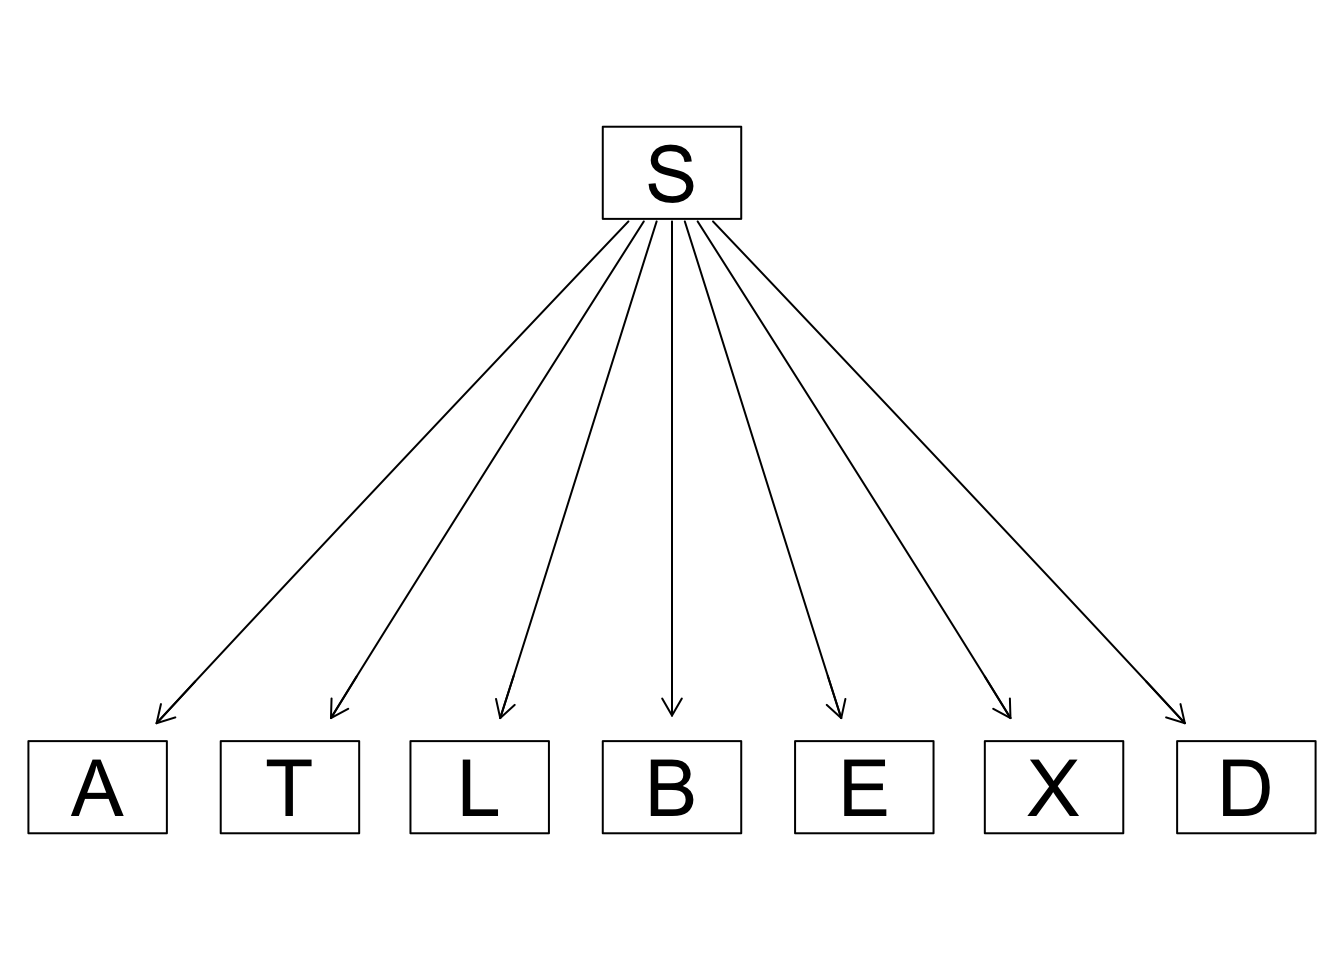
\includegraphics{oct2020_files/figure-latex/unnamed-chunk-4-1.pdf}

\begin{Shaded}
\begin{Highlighting}[]
\NormalTok{q\_table }\OtherTok{\textless{}{-}} \FunctionTok{array}\NormalTok{(}\DecValTok{0}\NormalTok{,}\AttributeTok{dim =} \FunctionTok{c}\NormalTok{(H,W,}\DecValTok{4}\NormalTok{))}
\NormalTok{   reward }\OtherTok{\textless{}{-}} \ConstantTok{NULL}
  \ControlFlowTok{for}\NormalTok{(i }\ControlFlowTok{in} \DecValTok{1}\SpecialCharTok{:}\DecValTok{5000}\NormalTok{) \{}
\NormalTok{    foo }\OtherTok{\textless{}{-}} \FunctionTok{q\_learning}\NormalTok{(}\AttributeTok{epsilon =} \FloatTok{0.5}\NormalTok{, }\AttributeTok{gamma =} \DecValTok{1}\NormalTok{, }\AttributeTok{start\_state =} \FunctionTok{c}\NormalTok{(}\DecValTok{1}\NormalTok{,}\DecValTok{1}\NormalTok{))}
\NormalTok{    reward }\OtherTok{\textless{}{-}} \FunctionTok{c}\NormalTok{(reward,foo[}\DecValTok{1}\NormalTok{])}
\NormalTok{  \}}

\FunctionTok{vis\_environment}\NormalTok{(i, }\AttributeTok{epsilon =} \FloatTok{0.5}\NormalTok{, }\AttributeTok{gamma =} \DecValTok{1}\NormalTok{, }\AttributeTok{alpha =} \FloatTok{0.1}\NormalTok{, }\AttributeTok{beta =} \DecValTok{0}\NormalTok{)}
\end{Highlighting}
\end{Shaded}

\includegraphics{oct2020_files/figure-latex/unnamed-chunk-4-2.pdf}

\begin{Shaded}
\begin{Highlighting}[]
\FunctionTok{plot}\NormalTok{(}\FunctionTok{MovingAverage}\NormalTok{(reward,}\DecValTok{100}\NormalTok{),}\AttributeTok{type =} \StringTok{"l"}\NormalTok{)}
\end{Highlighting}
\end{Shaded}

\includegraphics{oct2020_files/figure-latex/unnamed-chunk-4-3.pdf}

\begin{Shaded}
\begin{Highlighting}[]
\CommentTok{\# report final q table and policy}
\end{Highlighting}
\end{Shaded}


\end{document}
